\documentclass{csse4400}

% \teachermodetrue

\usepackage{float}

\usepackage{languages}

\title{Storing Stuff}
\author{Brae Webb}

\date{\week{3}}
\begin{document}

\maketitle

\begin{figure}[h]
  \href{https://www.oreilly.com/library/view/designing-data-intensive-applications/9781491903063/ch02.html}{
    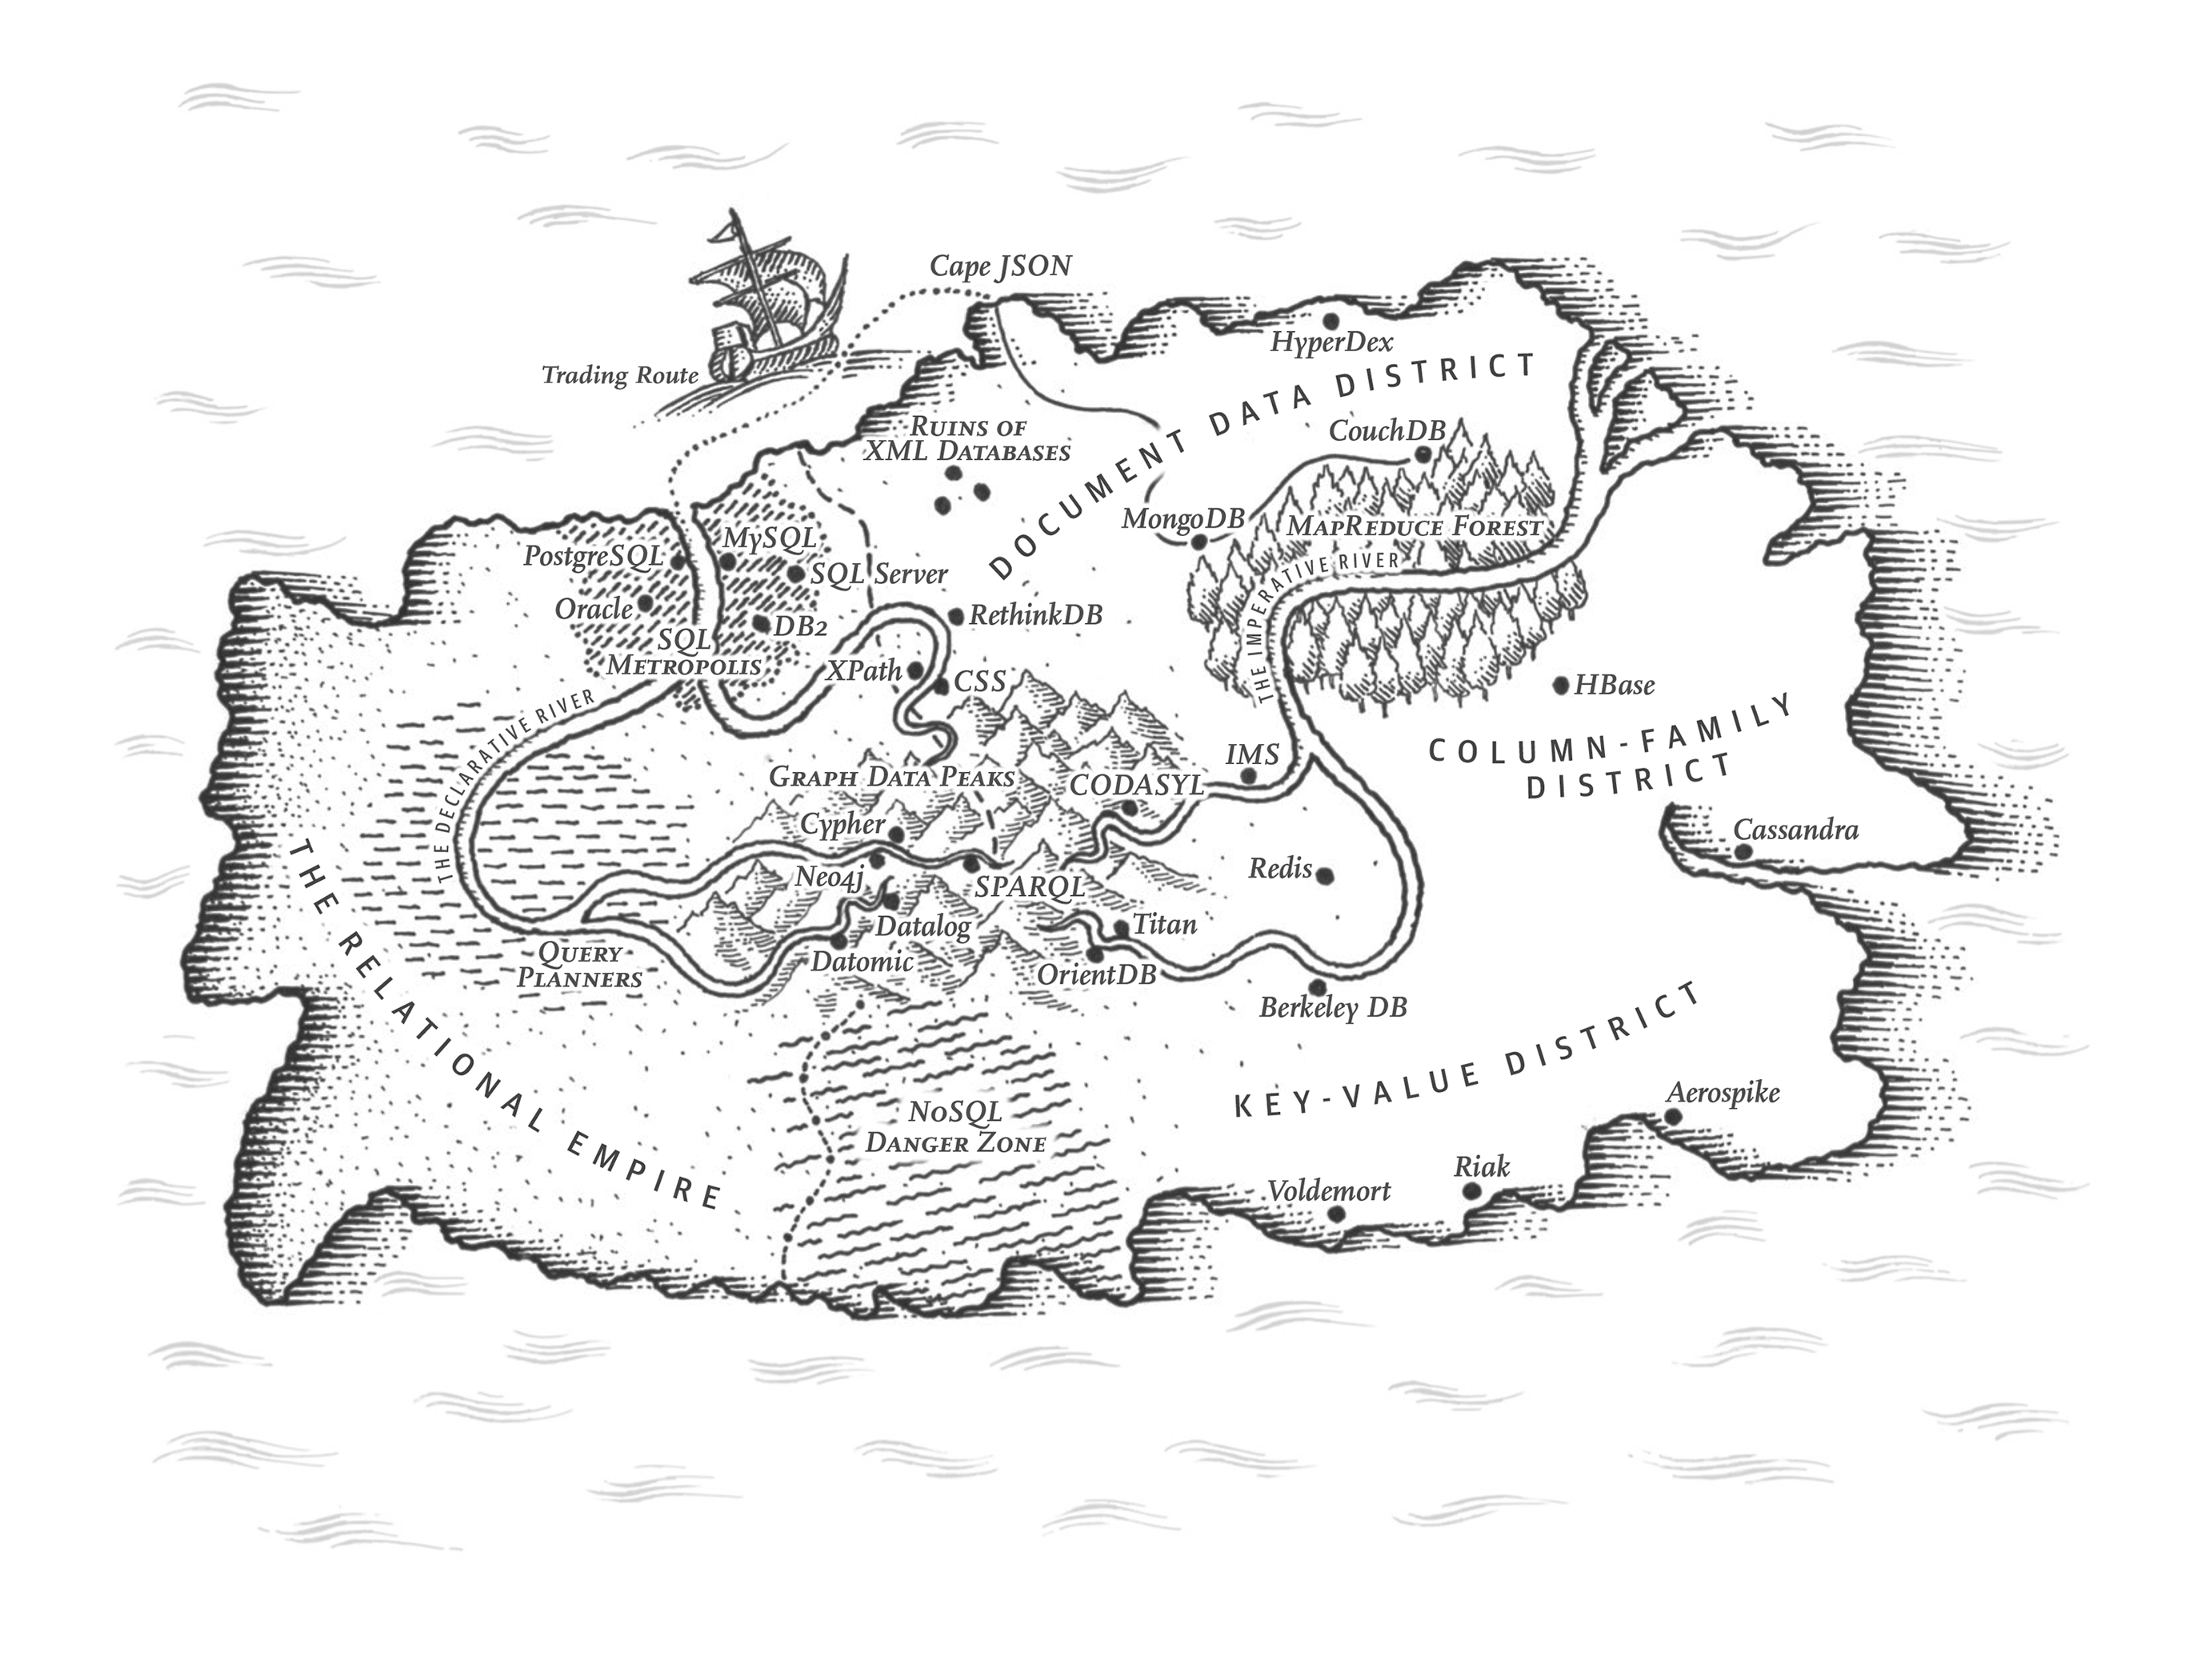
\includegraphics[width=\textwidth]{images/databases}
  }
\caption{A map of data storage techniques from Designing Data-Intensive Applications \cite{data-intensive}.}
\end{figure}

\section{This Week}
This week our goal is to:
\begin{itemize}
  \item explore the various techniques developers use to store data;
  \item investigate the storage options implementing these techniques on the AWS platform;
  \item run a small application using docker that requires a database; and
  \item deploy the application in AWS using Terraform.
\end{itemize}

\section{Databases and Data Models}
Unfortunately, to build interesting software we often need to store and use data.
The storage of data introduces a number of challenges when designing, creating, and maintaining our software.
However, not all data storage techniques are created equal;
the choice of data storage model can have a profound impact on our software's complexity and maintainability.
In this practical, we want to take a superficial exploration of our island of data storage models.
For a more in-depth treatment of data storage models that is outside the scope of this course,
see Chapter 2 of the \textit{Designing Data-Intensive Applications} book \cite{data-intensive}.

\teacher{
  Discuss the following different storage technologies and mention some use cases of when you would choose each one.
  Discuss some popular implementations of each.\\

  Aim for no more than 30 minutes of discussion.
}

\subsection{Relational Storage}

Relational databases what have been exposed to the most in your University career --- think MySQL, Postgres, Oracle DB, etc.
This type of database is good at modelling the real world which is often a highly connected environment.
% The data model that is suggested for this type of storage is a normalised approach where data duplication should be reduced.

Some popular offerings are below:

\begin{itemize}
  \item MySQL/MariaDB [ Amazon RDS / Amazon Aurora ].
  \item Postgres [ Amazon RDS / Amazon Aurora ].
\end{itemize}

The AWS offerings of these services come in two different types, we have the traditional approach of
server capacity ( x cores, y ram ) and we have a server-less approach.
The server-less approach is a more dynamic
database that can scale to large amounts of load when needed though at a cost per request.

  \subsubsection{ORM}
  Object Relational Mapping (ORM) is a fairly common tool for programmers to use to make developing with databases smoother.
  One fairly prevalent example of this is SQLAlchemy which is a very widely used 
  database abstraction for python.
  SQLAlchemy allows us to move to a higher level of abstraction than SQL queries and perform database actions using standard python code.

  The benefits of ORMs are the ability to model database objects in our existing programming language instead of having large blocks of SQL text within our source code.
  The disadvantages come in when we need to do specific SQL work or where the abstractions cost is greater than the benefits.

\subsection{Wide-Column Storage}

\teacher{
  Examples of big apps that depend on this technology is Netflix \url{https://netflixtechblog.com/netflixs-viewing-data-how-we-know-where-you-are-in-house-of-cards-608dd61077da}.
}

Wide-Column databases are a form of NoSQL or non-relational data stores.
In these data stores the data model design 
is focused more on having efficient queries at the cost of data duplication.
A warning to the reader that these models
are not flexible after creation, it is much easier to answer a new use case in a relational model.

  \begin{itemize}
    \item Apache Cassandra [ Amazon Keyspaces for Cassandra ].
    \item Apache HBase.
  \end{itemize}

\subsection{Key-Value Storage}

Key-Value stores are very popular for cache or remote config use cases, some of the most notable are Redis and Memcached.
These stores allow efficient lookup of values via keys and are usually stored in-memory.

\begin{itemize}
  \item Redis [ Amazon ElastiCache for Redis ].
  \item Memcached [ Amazon ElastiCache for Memcached].
  \item Amazon DynamoDB.
  \item Amazon MemoryDB for Redis.
\end{itemize}

\subsection{Time Series Storage}

\teacher{
  Something to mention here is that relations are usually not utilised between tables in time series databases.
}

Time series databases are highly focused storage which is tailored to retrieving results by timestamp ranges.
Many implementations also take advantage of the data model to allow efficient rollover of data and partitioning.
One of the most popular time series databases is Prometheus which is used to store monitoring metrics.

\begin{itemize}
  \item Amazon Timestream.
  \item TimescaleDB ( Postgres + Addon ).
  \item Prometheus.
  \item InfluxDB.
\end{itemize}

\subsection{Document Storage}

Document databases are a subset of NoSQL databases with a focus on a flexible data model.
MongoDB for instance allows the user to store JSON documents and perform queries on those documents.
One advantage of document databases is that they match a programmers existing mental model of storing data in formats such as JSON.

\begin{itemize}
  \item MongoDB.
  \item Apache CouchDB.
  \item Amazon DocumentDB.
  \item Amazon DynamoDB.
\end{itemize}

\subsection{Graph Storage}

\teacher{
  If you havnt experienced graph databases, a good usecase is ``recommendation systems'',
  which use the connected nature of items to figure out what to suggest to a person.Another example is the \url{https://neo4j.com/blog/analyzing-panama-papers-neo4j/}
  Panama Papers.
}

Graph Databases are relational storage with a few enhancements to allow fast neighbour look-ups.
These databases also allow the implementation of graph algorithms to query data.

\begin{itemize}
  \item Amazon Neptune.
  \item Neo4J.
  \item Janus Graph.
\end{itemize}

\section{Working with Docker}

So far in the course we have introduced docker as a means to package software to make it easier to work with and deploy.
Today we will be using it to run a small application locally that consists of a web server and a relational database.

\begin{figure}[H]
  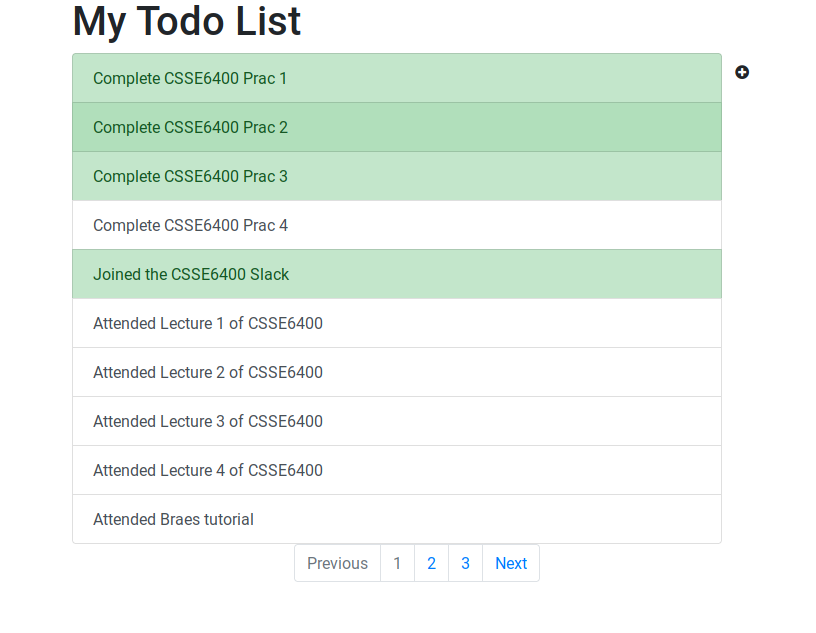
\includegraphics[width=\textwidth]{images/todoapp}
\caption{Sample Todo App made by Brae Webb}
\end{figure}

\info{
    You will need to have docker and docker-compose installed for this practical.
    Installation will depend on your operating system.

    \begin{itemize}
      \item Docker compose: https://docs.docker.com/compose/install/
      \item Docker engine: https://docs.docker.com/get-docker/
    \end{itemize}
    
    We also recommend installing the vscode docker plugin or the equlivant tools in IntelliJ IDEs.
}

\teacher{
  Wait for students to get docker-compose installed,
  they should have docker from their tutorials but some may be missing it.
}

\notice{
    For terminal examples in this section,
    lines that begin with a \$ indicate a line which you should type while the other lines are example output that you should expect.
    Not all of the output is captured in the examples to save on space.  
}

\subsection{Locally}

\teacher{
  Mention that the dockerfile exists but no need to get the repo.
  We will not be building the container ourselves.
  Instead use one that is published on the github,
  shown further down in the docker-compose.
}

We will be using a container that is built from the Dockerfile described below which can be found here: 
\url{https://github.com/CSSE6400/todo-app/blob/main/backend/Dockerfile}.

\begin{code}[language=docker]{Dockerfile}
FROM ubuntu:21.10
RUN apt-get update \
        && DEBIAN_FRONTEND=noninteractive apt install -y \
            php \
            php-mysql \
            php-xml \
            php-curl \
            curl \
            git \
            unzip
RUN curl -sS https://getcomposer.org/installer | php -- --install-dir=/usr/local/bin --filename=composer
COPY . /app
WORKDIR /app
RUN composer install
CMD ["php", "artisan", "serve", "--host=0.0.0.0"]
\end{code}

Our goal for today is to have a running instance of the Todo App locally including the database.
To get started we need to make a new directory for our work and create a Docker compose file.

\begin{code}[language=shell,numbers=none]{}
  $ mkdir prac4 && cd prac4
  $ touch docker-compose.yml
\end{code}

Docker Compose is a small helper utility that allows us to more easily run docker applications without needing to remember a lot of command line parameters.
Instead we define how we want our docker container to run through a YAML config file.
Insert the following into your docker-compose.yml file.

\begin{code}[language=docker-compose]{docker-compose.yml}
version: '3.3'
services:
  backend:
    image: ghcr.io/csse6400/todo-app:latest
    ports:
      - '8000:8000'
    environment:
      APP_ENV: 'local'
      APP_KEY: 'base64:8PQEPYGlTm1t3aqWmlAw/ZPwCiIFvdXDBjk3mhsom/A='
      APP_DEBUG: 'true'
      LOG_LEVEL: 'debug'
\end{code}

\teacher{
  Feel free to show students dockerhub and where on github this container is stored. URL for 
  this container is here \url{https://github.com/CSSE6400/todo-app/pkgs/container/todo-app}
}

A few things to point out in the file.
We have defined a single service called backend which uses a pre-made docker image from \url{ghcr.io/csse6400/todo-app} with the tag of latest.
We then have exposed this onto our machine on port 8000 and have passed a few environment variables.%\lstinline{docker-compose up}.

\begin{code}[language=shell,numbers=none]{}
  $ docker-compose up
  Creating network "p1_default" with the default driver
  Creating p1_backend_1 ... done
  Attaching to p1_backend_1
  backend_1  | Starting Laravel development server: http://0.0.0.0:8000
  backend_1  | [Sun Mar 20 07:56:23 2022] PHP 8.0.8 Development Server (http://0.0.0.0:8000) started
\end{code}

Now we head to our browser and go to \url{http://127.0.0.1:8000},
you should be presented with the following screen.

\begin{figure}[ht]
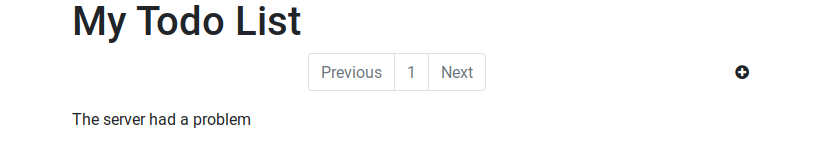
\includegraphics[width=\textwidth]{images/app-missing-db}
\end{figure}

To investigate this error lets hit one of the endpoints for our api.
Head over to \url{http://127.0.0.1:8000/api/v1/todo} which should list all the todos.
Once we reach that page we have a clearer idea of whats gone wrong.
The page you should see is shown in Figure \ref{fig:expected-error} and the quick summary is that our App is complaining that we haven't given it a database.

\begin{figure}[H]
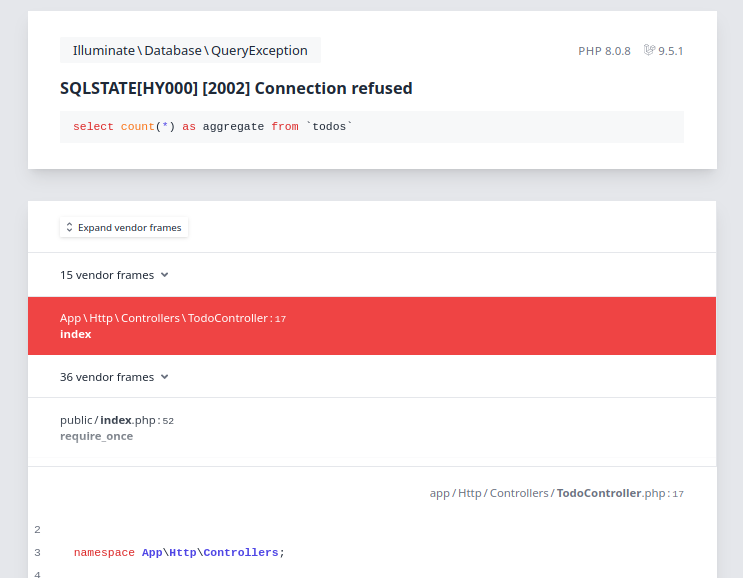
\includegraphics[width=\textwidth]{images/missing-db}
\caption{The expected error page when accessing \url{http://127.0.0.1:8000/api/v1/todo}.}
\label{fig:expected-error}
\end{figure}

To fix this lets add a popular relation database, MySQL, to our docker-compose file.
Edit your docker compose file to match as shown below.

\begin{code}[language=docker-compose]{main.tf}
version: '3.3'
services:
  db:
    image: mysql:8-debian
    environment:
      MYSQL_DATABASE: 'todoapp'
      MYSQL_USER: 'todoapp'
      MYSQL_PASSWORD: 'password'
      MYSQL_ROOT_PASSWORD: 'password'
    ports:
      - '3306:3306'

  backend:
    image: ghcr.io/csse6400/todo-app:latest
    depends_on:
      - db
    ports:
      - '8000:8000'
    environment:
      APP_ENV: 'local'
      APP_KEY: 'base64:8PQEPYGlTm1t3aqWmlAw/ZPwCiIFvdXDBjk3mhsom/A='
      APP_DEBUG: 'true'
      LOG_LEVEL: 'debug'
      DB_CONNECTION: 'mysql'
      DB_HOST: 'db'
      DB_PORT: '3306'
      DB_DATABASE: 'todoapp'
      DB_USERNAME: 'todoapp'
      DB_PASSWORD: 'password'
\end{code}

Now we have two services for our app and we have added a few more environment variables for our backend to know how to connect to the database.
The \texttt{DB\_HOST} variable uses a feature of docker compose where you can refer to other services by their name.
This makes it easy for us to setup communication between these two services.

From the same shell let's re-run our containers,
you may need to CTRL+C to stop the current running containers.
Once they have shutdown, run the up command again.

\begin{code}[language=shell,numbers=none]{}
  $ docker-compose up
  Starting p2_db_1 ... done
  Starting p2_backend_1 ... done
  Attaching to p2_db_1, p2_backend_1
  db_1       | 2022-03-20 08:11:55+00:00 [Note] [Entrypoint]: Entrypoint ....
  db_1       | 2022-03-20 08:11:55+00:00 [Note] [Entrypoint]: Switching t....
  db_1       | 2022-03-20 08:11:55+00:00 [Note] [Entrypoint]: Entrypoint ....
  db_1       | 2022-03-20T08:11:55.438996Z 0 [System] [MY-010116] [Server....
  db_1       | 2022-03-20T08:11:55.445261Z 1 [System] [MY-013576] [InnoDB....
  backend_1  | Starting Laravel development server: http://0.0.0.0:8000
  db_1       | 2022-03-20T08:11:55.535803Z 1 [System] [MY-013577] [InnoDB....
  db_1       | 2022-03-20T08:11:55.673757Z 0 [Warning] [MY-010068] [Serve....
  db_1       | 2022-03-20T08:11:55.673784Z 0 [System] [MY-013602] [Server....
  db_1       | 2022-03-20T08:11:55.674810Z 0 [Warning] [MY-011810] [Serve....
  db_1       | 2022-03-20T08:11:55.684729Z 0 [System] [MY-010931] [Server....
  db_1       | 2022-03-20T08:11:55.684756Z 0 [System] [MY-011323] [Server....
  backend_1  | [Sun Mar 20 08:11:55 2022] PHP 8.0.8 Development Serv....
\end{code}

Now when we go to \url{http://127.0.0.1:8000/api/v1/todo} we see a different error message, as shown in Figure \ref{fig:missing-tables}.
This error is complaining that we have a database that we can connect to but the todos table doesn't exist.

\begin{figure}[ht]
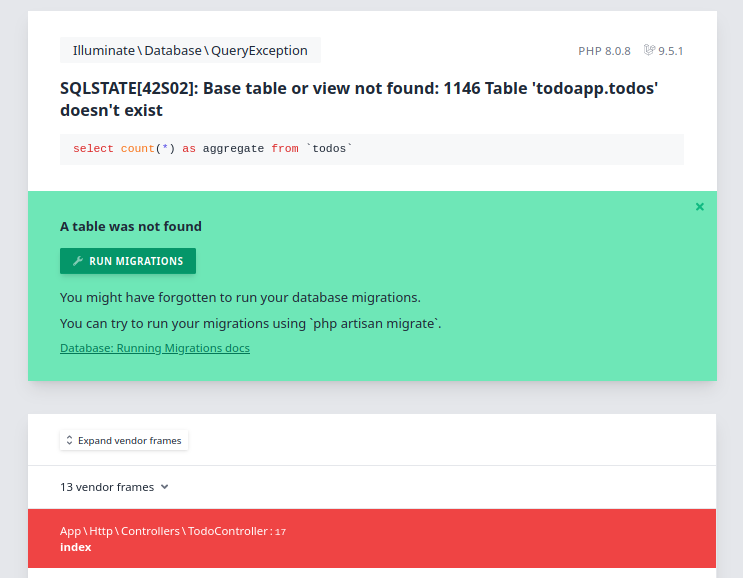
\includegraphics[width=\textwidth]{images/missing-tables}
\caption{The expected error page when accessing \url{http://127.0.0.1:8000/api/v1/todo} after creating a database.}
\label{fig:missing-tables}
\end{figure}

To populate the database our application comes with database migration files.
One way would be to click the ``RUN MIGRATIONS'' button shown on the error page but we also want to pre-populate our database with some dummy data as well.

To do this we are going to jump into the running container and execute the migrations ourselves.
Start by opening a new terminal so that we can leave the docker containers running.
In this new terminal go to the same directory that we were just in and run the following 
command:

\begin{code}[language=shell,numbers=none]{}
$ docker-compose exec backend php artisan migrate:fresh --seed
Dropped all tables successfully.
Migration table created successfully.
Migrating: 2022_03_19_041557_create_todos_table
Migrated:  2022_03_19_041557_create_todos_table (7.55ms)
Seeding: Database\Seeders\TodoSeeder
Seeded:  Database\Seeders\TodoSeeder (6.56ms)
Database seeding completed successfully.
\end{code}

\noindent Now with this run we can check back at our web app and you should see a fully 
functional todo app.

\begin{figure}[ht]
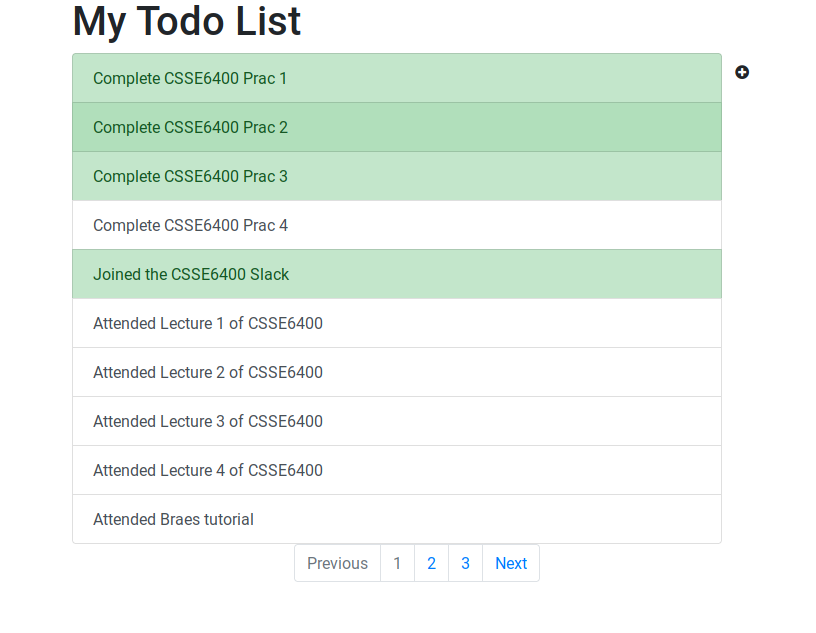
\includegraphics[width=\textwidth]{images/todoapp}
\end{figure}

\info{
  These migrations are performed by Laravel which is a popular PHP web framework.
  In the database it has created a table to keep track of which migrations have already been run so that it will skip them latter.
  To enable this functionality you will have to edit migrate:fresh to just migrate.\\

  For a production instance you would also typically remove the --seed parameter as you do not want to insert dummy data into your production database.
}

\subsubsection{Exercise: Migrations at startup}

So far when we run this application we have to perform the database migrations manually. 
To help us get up and running we are going to make a small modification to pre-run the migrations when are web app starts.
First we need to have a look at how the container is set to launch by default.
In the Dockerfile attached at the start of the practical we see that we have defined the command to run on the last line with the CMD directive.

\begin{code}[language=docker]{Dockerfile}
  FROM ubuntu:21.10
  ... 
  ... 
  ...
  CMD ["php", "artisan", "serve", "--host=0.0.0.0"]
\end{code}

\info{
  When working with docker it can get confusing around the networking aspects. In this application I have specified
  that the server must listen on all network interfaces ( 0.0.0.0 ). Without this flag the default is 127.0.0.1 which
  even though its the localhost the forwarded traffic through the docker container would never reach it.
}

This command launches the laravel development server and listens on all interfaces on the host.
We are going to override this in our docker-compose file so that we run the migrations then start the server.
Add the following line to the docker-compose.yml that you have been developing during the practical.

\begin{code}[language=docker-compose]{}
  command: sh -c "sleep 30 && php artisan migrate:refresh --seed && php artisan serve --host=0.0.0.0"
\end{code}

This new command does the following:

\begin{itemize}
  \item Waits for the database to be ready in a simple way.
  \item Runs the migrations and seeds the database, as we have seen earlier.
  \item Starts the development server as the container originally did.
\end{itemize}

Example: condensed version of the goal \texttt{docker-compose.yml} attached below.

\begin{code}[language=docker-compose]{docker-compose.yml}
  version: '3.3'
  services:
    db:
      ...
  
    backend:
      ...
      environment:
        ...
      command: sh -c "sleep 10 && php artisan migrate:refresh --seed && php artisan serve --host=0.0.0.0"
\end{code}

Now when we launch the docker-compose we can see that our migrations were run in the output.

\begin{code}[language=shell,numbers=none]{}
  $ docker-compose up
  ...
  ...
  backend_1  | Rolling back: 2022_03_19_041557_create_todos_table
  backend_1  | Rolled back:  2022_03_19_041557_create_todos_table (8.28ms)
  backend_1  | Migrating: 2022_03_19_041557_create_todos_table
  backend_1  | Migrated:  2022_03_19_041557_create_todos_table (11.55ms)
  backend_1  | Seeding: Database\Seeders\TodoSeeder
  backend_1  | Seeded:  Database\Seeders\TodoSeeder (44.77ms)
  backend_1  | Database seeding completed successfully.
  backend_1  | Starting Laravel development server: http://0.0.0.0:8000
  backend_1  | [Sun Mar 20 12:08:41 2022] PHP 8.0.8 Development Server (http://0.0.0.0:8000) started
\end{code}

We can also bake this into the container by extending the original,
it is fairly common to see projects in the wild that run a init script when the container launches.
An exercise left for the reader is to build upon the provided docker container by including an init script.

\subsection{AWS}

\warning{
  This section is still being developed.
}

\bibliographystyle{ieeetr}
\bibliography{books}

\end{document}